\section{Dataset Characteristics}

\subsection{KL3M Components and Summary Statistics}
While currently limited mostly to governmental sources, the KL3M dataset features a relatively large and diverse set of content such as the content highlighted in Figure \ref{fig:KL3MImages}.  In Table \ref{table:summarystats}, we present summary statistics for the overall dataset.  In total, the KL3M dataset features more than 125 million documents, 1.7 trillion tokens and more than 80 terabyte of total information content.  

\begin{table}[!htbp]
    \small
    \centering
    \begin{tabularx}{0.6\linewidth}{X @{\hskip 3pt} l @{\hskip 3pt}}
        \toprule
        \textbf{KL3M Features} & \\
        \midrule
        Total Documents in KL3M & 126 Million Documents \\
        Total Tokens in KL3M  & 1.7 Trillion Tokens \\
        Total File Size & 80 Terabytes \\
        \midrule
        \bottomrule
    \end{tabularx}
    \caption{Summary Statistics for KL3M Dataset}
    \label{table:summarystats}
\end{table}

Given the range of sources as the vast interconnectedness of ideas, concepts, there is almost certainly duplicate content contained herein. A document may quote elements of other documents or otherwise incorporate concepts from other documents.  Thus, the overall token count is somewhat larger than if one were to consider something such as the total number unique n-gram combinations.  However, we did not deduplicate the underlying content as we envision a wide range of potential uses for this overall source material.  Downstream users can thus decide how to mix, match, segment or further pre-process the content in order to support their specific objective or use case.  

\begin{table}[!htbp]
   \footnotesize
  \centering 
    \begin{tabular*}{\linewidth}{Xlrrr|r}
    \toprule
    \textbf{KL3M Component}  & {\sc{File Size}} & {\sc Document Count} & {\sc Token Count} & {\sc Avg Token Per Doc}\\
    \midrule
    Securities \& Exchange Commission Filings & 00.0GiB & 0.0 & 0.0 & 0.0 \\
Congressional Documents & 00.0GiB & 0.0  & 0.0 & 0.0 \\
Congressional Bills & 00.0GiB & 0.0  & 0.0 & 0.0 \\
Code of Federal Regulations &  00.0GiB & 0.0 & 0.0 & 0.0 \\
Electronic Code of Federal Regulations &  00.0GiB & 0.0  & 0.0 & 0.0  \\
Federal Depository Library Program &  00.0GiB & 0.0 & 0.0 & 0.0  \\
Federal Register &  00.0GiB & 0.0  & 0.0 & 0.0 \\
Federal Judicial Center &  00.0GiB & 0.0 & 0.0 & 0.0  \\
CIA World Factbook &  00.0GiB & 0.0  & 0.0 & 0.0  \\
Congressional Research Service &  00.0GiB & 0.0 & 0.0 & 0.0 \\
United States Government Manual &  00.0GiB & 0.0 & 0.0 & 0.0 \\
Library of Congress - Country Profiles &  00.0GiB & 0.0 & 0.0 & 0.0 \\
Statutes at Large &  00.0GiB & 0.0  & 0.0 & 0.0 \\
Regulatory Submissions &  00.0GiB & 0.0 & 0.0 & 0.0 \\
United States Code &  00.0GiB & 0.0 & 0.0 & 0.0 \\
Court Documents - Opinions &  00.0GiB & 0.0 & 0.0 & 0.0 \\
Court Documents - Motions, Orders, etc. &  00.0GiB & 0.0 & 0.0 & 0.0\\
Court Documents - Dockets  &  00.0GiB & 0.0  & 0.0 & 0.0 \\
Black's Law Dictionary, 2nd Edition &  00.0GiB & 0.0 & 0.0 & 0.0 \\
U.S. Federal Government Websites &  00.0GiB & 0.0 & 0.0 & 0.0 \\
US Patent Grant Full Text Data &  00.0GiB & 0.0  & 0.0 & 0.0 \\
Official Journal of the European Union &  00.0GiB & 0.0 & 0.0 & 0.0 \\
    \midrule
    \textbf{Totals} & \textbf{0.0} & \textbf{0.0} & \textbf{0.0} & \textbf{0.0}   \\
    \bottomrule
    \end{tabular*}%
  \label{table:KL3M Components}%
      \caption{Summary Statistics of KL3M Components }
\end{table}

Table \ref{table:summarystats} displays the document counts, token counts and average tokens per document for each of the KL3M components.  While \textit{Securities \& Exchange Commission Filings} are the largest component of the dataset from a total documents and token perspective, there are some other large sources of input data.  Other large subset of data include [ FILL IN NEXT 3-4 items]  

Among some of the smaller KL3M components, there are interesting elements worthy of exploration including millions of conversational messages extracted from Congressional hearings, nearly 20 billion tokens worth of docket entiries 

Appendix II offers a more detailed description of each of the KL3M Components.  




\subsection{KL3M Additional Compositional Statistics}

\textbf{DISTRIBUTION OF DOCUMENT SIZE}

\begin{figure}[h!]
\centering
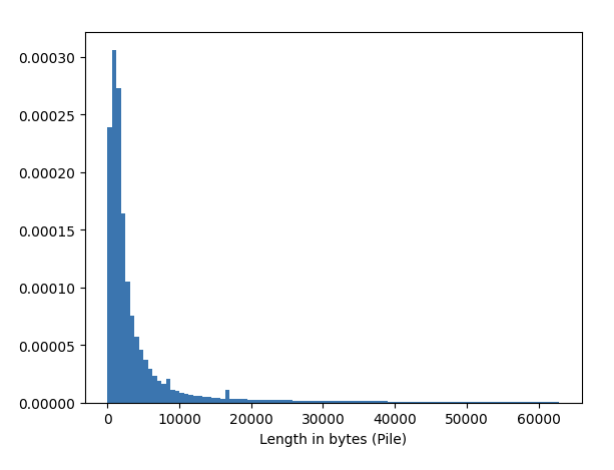
\includegraphics[width=90mm]{PileDist.png}
\caption{\centering{{Overview of the Pre-Processing Pipeline} - (icons via Flaticon)}}
\label{fig:Dist}
\end{figure}


\textbf{DISTRIBUTION OF PERPLEXITY SCORES}
\begin{figure}[h!]
\centering
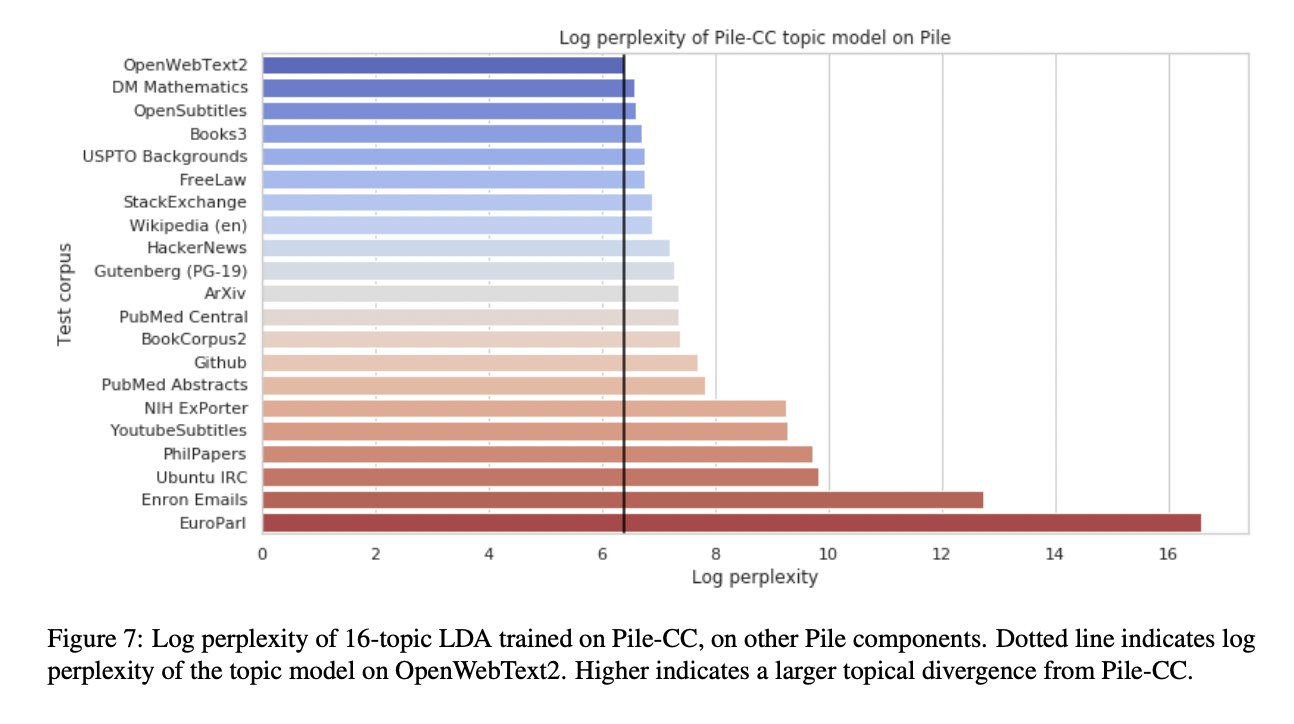
\includegraphics[width=110mm]{Perplexity.png}
\caption{\centering{{Overview of the Pre-Processing Pipeline} - (icons via Flaticon)}}
\label{fig:Perplexity}
\end{figure}


\textbf{TOXICITY ANALYSIS}
\begin{figure}[h!]
\centering
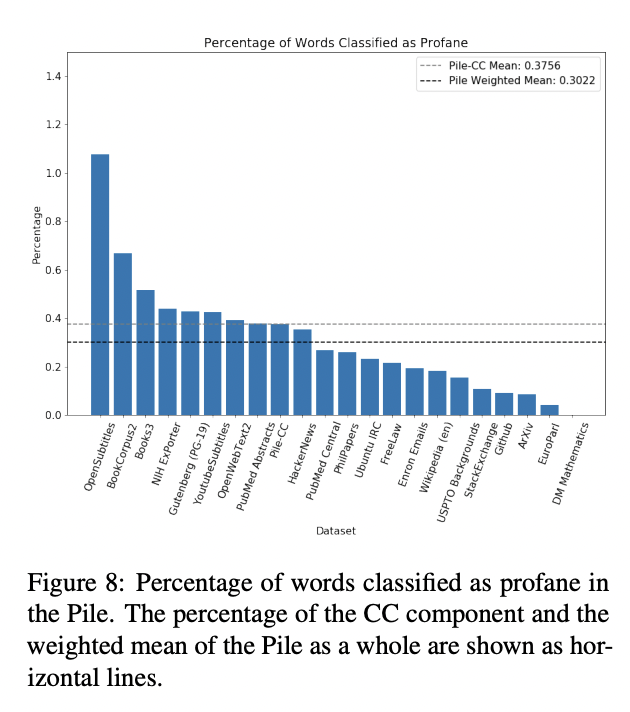
\includegraphics[width=90mm]{Toxicity.png}
\caption{\centering{{Overview of the Pre-Processing Pipeline} - (icons via Flaticon)}}
\label{fig:toxicity}
\end{figure}




Trying to copy some of the stuff reported in THE PILE paper 

\textbf{TOTAL TOKENS }

\vspace{10mm}

\textbf{TOTAL DOCS (with cavaet and discussion that doc is a tricky idea)}

\vspace{10mm}

\textbf{DISTRIBUTION OF TOKENS by Docs}

\vspace{10mm}

\textbf{SOME SORT OF TOKEN DIVERSITY MEASURE }

\vspace{10mm}





\textbf{Why US other countries -- data availability .. 
}




